\documentclass[a4paper,10pt]{jsarticle}

% 数式
\usepackage{amsmath,amsfonts}
\usepackage{bm}
% 画像
\usepackage[dvipdfmx]{graphicx}
\usepackage{here}

\usepackage{listingsutf8,jlisting} %日本語のコメントアウトをする場合jlistingが必要
%ここからソースコードの表示に関する設定
\lstset{
  basicstyle={\ttfamily},
  identifierstyle={\small},
  commentstyle={\smallitshape},
  keywordstyle={\small\bfseries},
  ndkeywordstyle={\small},
  stringstyle={\small\ttfamily},
  frame={tb},
  breaklines=true,
  columns=[l]{fullflexible},
  numbers=left,
  xrightmargin=0zw,
  xleftmargin=3zw,
  numberstyle={\scriptsize},
  stepnumber=1,
  numbersep=1zw,
  lineskip=-0.5ex
}

\begin{document}

\title{生体情報処理課題3}
\author{坪井正太郎(101830245)}
\date{\today}
\maketitle
\section{}
C++で実装した。
標準ライブラリで乱数を生成し、初期の重みを設定した。
$\lambda$は1として、2乗誤差が0.001以下になるように学習させた。

\begin{figure}[H]
  \centering
  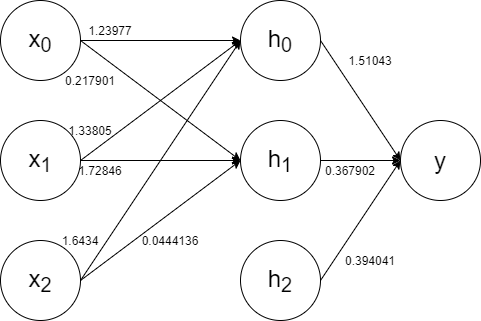
\includegraphics[width=10cm]{01.png}
  \caption{初期状態}
\end{figure}

学習後の出力は以下の通り
\[f(00)=0.950596\]
\[f(01)=0.0426667\]
\[f(10)=0.0427868\]
\[f(11)=0.956396\]

\begin{figure}[H]
  \centering
  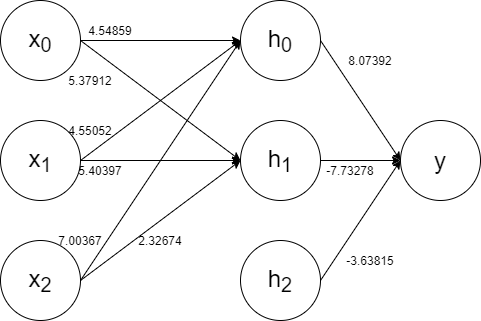
\includegraphics[width=10cm]{02.png}
  \caption{学習後}
\end{figure}

\end{document}
